\begin{figure}[p]\centering
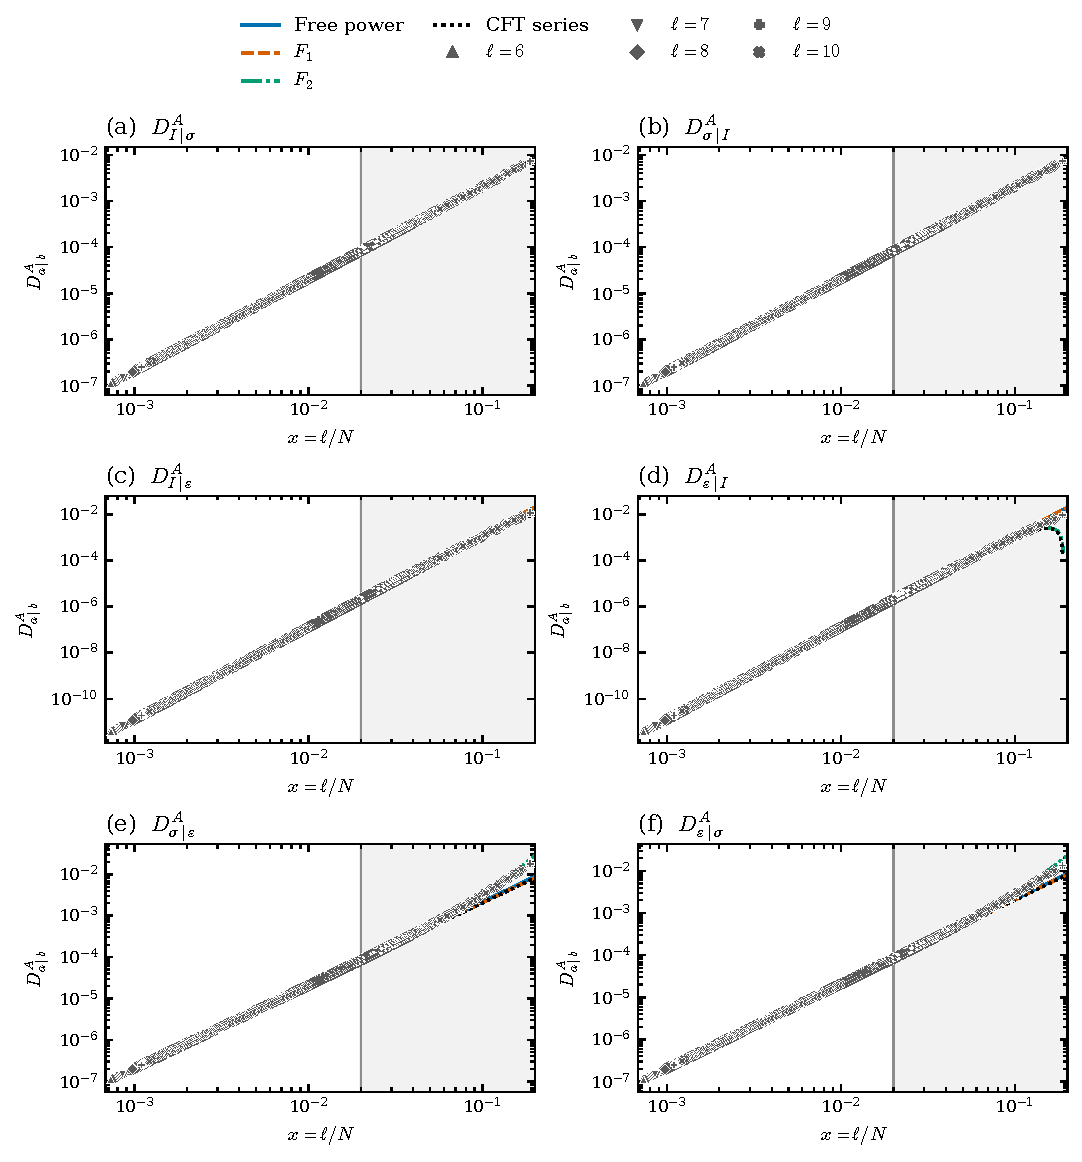
\includegraphics[width=.88\linewidth]{../figs/ising_small_value.pdf}
\caption{Both axes are logarithmic. Nonpositive values of an extrapolated truncated curve are omitted only from this logarithmic panel, while residual panels retain their predictions. Ising mixtures at $p=1/2$, $\ell=6,7,8,9,10$, and the chain-size set in Eq.~\eqref{eq:extended-grid}, with $32\leq N\leq8192$. There are 1645 displayed geometries per direction at $x\leq0.2$, of which 1255 satisfy $x\leq0.02$ and enter every fit. Marker shape identifies $\ell$; the vertical boundary and gray shading mark the fitting cutoff and excluded data. The periodic Ising Hamiltonian is $H=-\sum_jX_jX_{j+1}-\sum_jZ_j$; primaries use exact fermionic covariances, including the odd Ramond ground state for $\sigma$. Natural logarithms apply. Added sizes use the direct entropy remainder in Sec.~\ref{sec:stable-entropy}, with support cutoff $10^{-15}$. Blue solid is the free-power fit (two fitted parameters), orange dashed is $F_1$ (one), green dash--dot is $F_2$ (two), and black dotted is the supplied CFT series (zero). Powers and amplitudes use Eqs.~\eqref{eq:fit} and \eqref{eq:hierarchy}; all coefficients include powers of $\pi$. Fits minimize unweighted squared residuals in $D^A$. These curves use \texttt{scaling\_fit\_summary.csv}. The identical fits in Tables~\ref{tab:ising-small-parameters} and \ref{tab:ising-small-metrics} also have per-pair full-range and fitting-window views in Sec.~\ref{sec:pair-small_ising}.}
\label{fig:isingfits}
\end{figure}

\begin{figure}[p]\centering
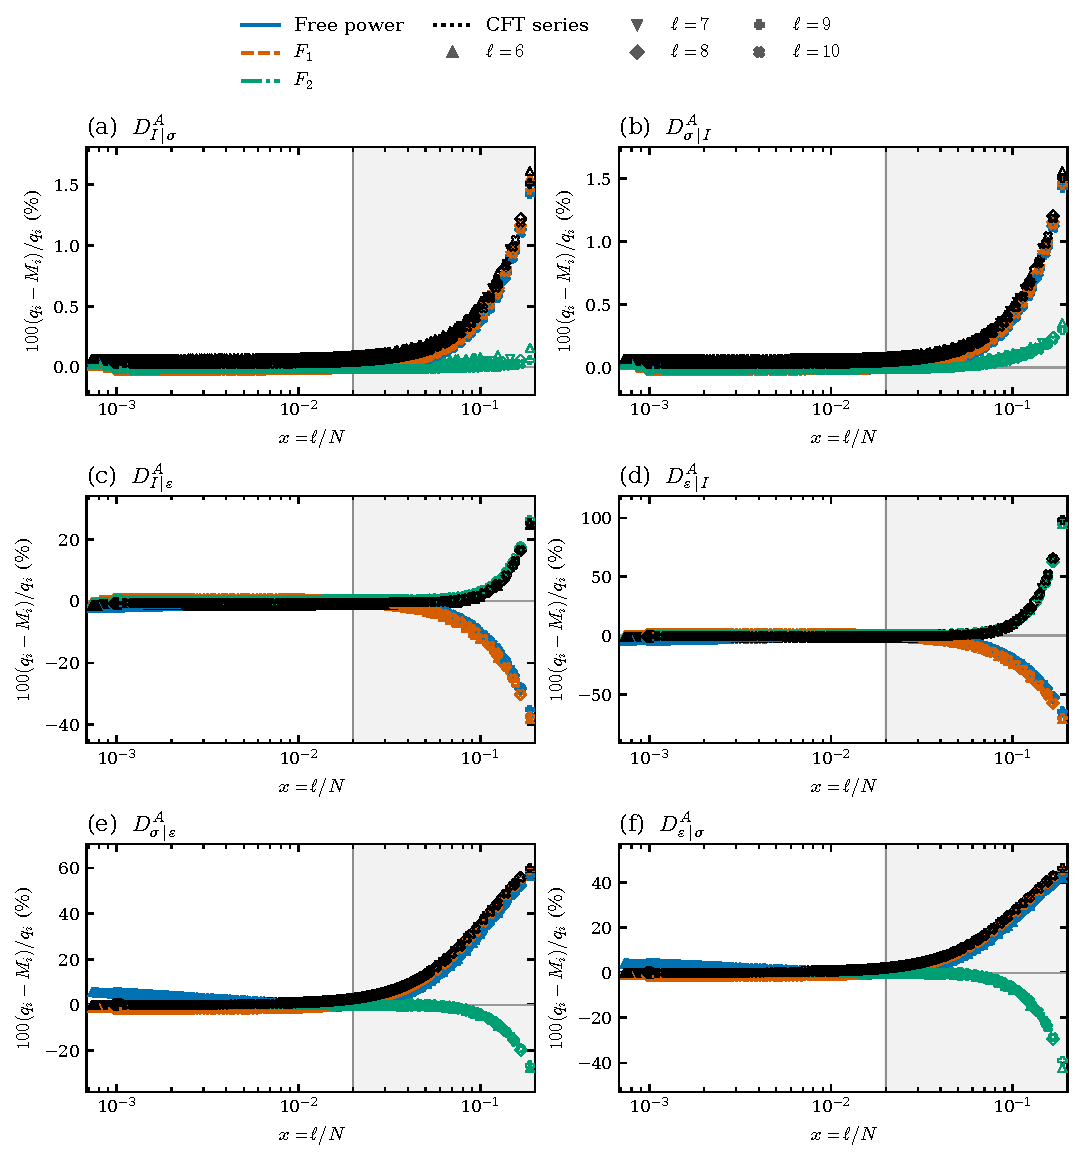
\includegraphics[width=.88\linewidth]{../figs/ising_small_residual.pdf}
\caption{The ordinate is $100(q_i-M_i)/q_i$ percent, with $q_i=D^A_i$ for a small interval and $q_i=\delta_i$ for a large interval; the horizontal zero line aids comparison. All four models have residual markers, colored as their curves. The residual ordinate is linear; the fraction axis is logarithmic. Ising mixtures at $p=1/2$, $\ell=6,7,8,9,10$, and the chain-size set in Eq.~\eqref{eq:extended-grid}, with $32\leq N\leq8192$. There are 1645 displayed geometries per direction at $x\leq0.2$, of which 1255 satisfy $x\leq0.02$ and enter every fit. Marker shape identifies $\ell$; the vertical boundary and gray shading mark the fitting cutoff and excluded data. The periodic Ising Hamiltonian is $H=-\sum_jX_jX_{j+1}-\sum_jZ_j$; primaries use exact fermionic covariances, including the odd Ramond ground state for $\sigma$. Natural logarithms apply. Added sizes use the direct entropy remainder in Sec.~\ref{sec:stable-entropy}, with support cutoff $10^{-15}$. Blue solid is the free-power fit (two fitted parameters), orange dashed is $F_1$ (one), green dash--dot is $F_2$ (two), and black dotted is the supplied CFT series (zero). Powers and amplitudes use Eqs.~\eqref{eq:fit} and \eqref{eq:hierarchy}; all coefficients include powers of $\pi$. Fits minimize unweighted squared residuals in $D^A$. These curves use \texttt{scaling\_fit\_summary.csv}. The identical fits in Tables~\ref{tab:ising-small-parameters} and \ref{tab:ising-small-metrics} also have per-pair full-range and fitting-window views in Sec.~\ref{sec:pair-small_ising}.}
\label{fig:isingresid}
\end{figure}

\begin{figure}[p]\centering
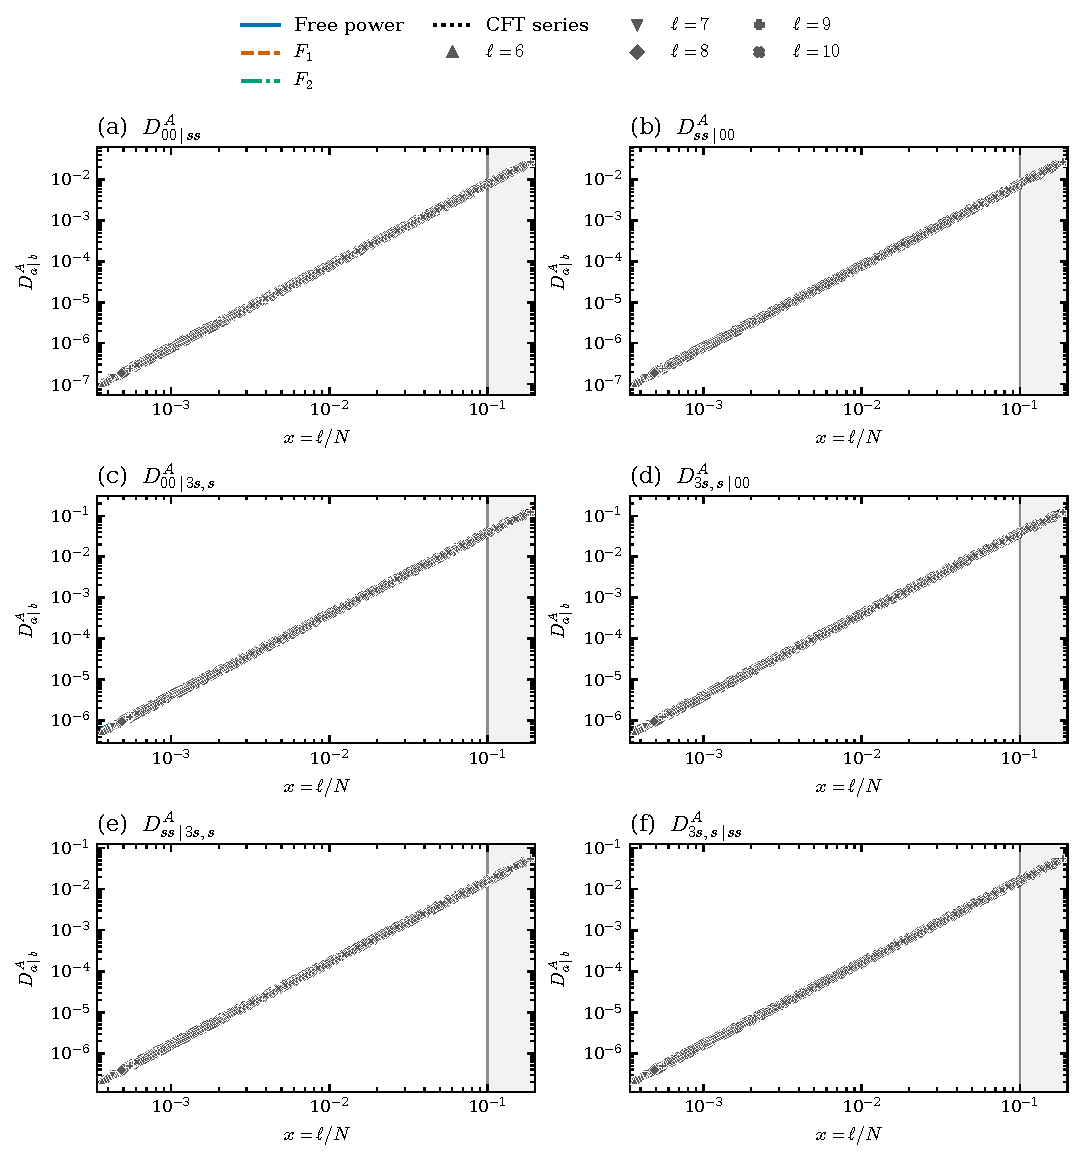
\includegraphics[width=.88\linewidth]{../figs/boson_small_value.pdf}
\caption{Both axes are logarithmic. Nonpositive values of an extrapolated truncated curve are omitted only from this logarithmic panel, while residual panels retain their predictions. Compact-boson mixtures at $p=1/2$, $\ell=6,7,8,9,10$, and the chain-size set in Eq.~\eqref{eq:extended-grid}, with $32\leq N\leq16384$. There are 625 displayed geometries per direction at $x\leq0.2$, of which 598 satisfy $x\leq0.1$ and enter every fit. Marker shape identifies $\ell$; the vertical boundary and gray shading mark the fitting cutoff and excluded data. The boson uses $s=1/\sqrt2$, $q=2$, charge codes $(0,0),(1,1),(3,1)$, $z_j=e^{2\pi i j/N}$, $w_1=0$, and $W=10^8$; moment algebra uses 100 digits through $N=256$ and 120 digits at the added sizes. Natural logarithms apply. Added sizes use the direct entropy remainder in Sec.~\ref{sec:stable-entropy}, with support cutoff $10^{-15}$. Blue solid is the free-power fit (two fitted parameters), orange dashed is $F_1$ (one), green dash--dot is $F_2$ (two), and black dotted is the supplied CFT series (zero). Powers and amplitudes use Eqs.~\eqref{eq:fit} and \eqref{eq:hierarchy}; all coefficients include powers of $\pi$. Fits minimize unweighted squared residuals in $D^A$. These curves use \texttt{scaling\_fit\_summary.csv}. The identical fits in Tables~\ref{tab:boson-small-parameters} and \ref{tab:boson-small-metrics} also have per-pair full-range and fitting-window views in Sec.~\ref{sec:pair-small_boson}.}
\label{fig:bosonfits}
\end{figure}

\begin{figure}[p]\centering
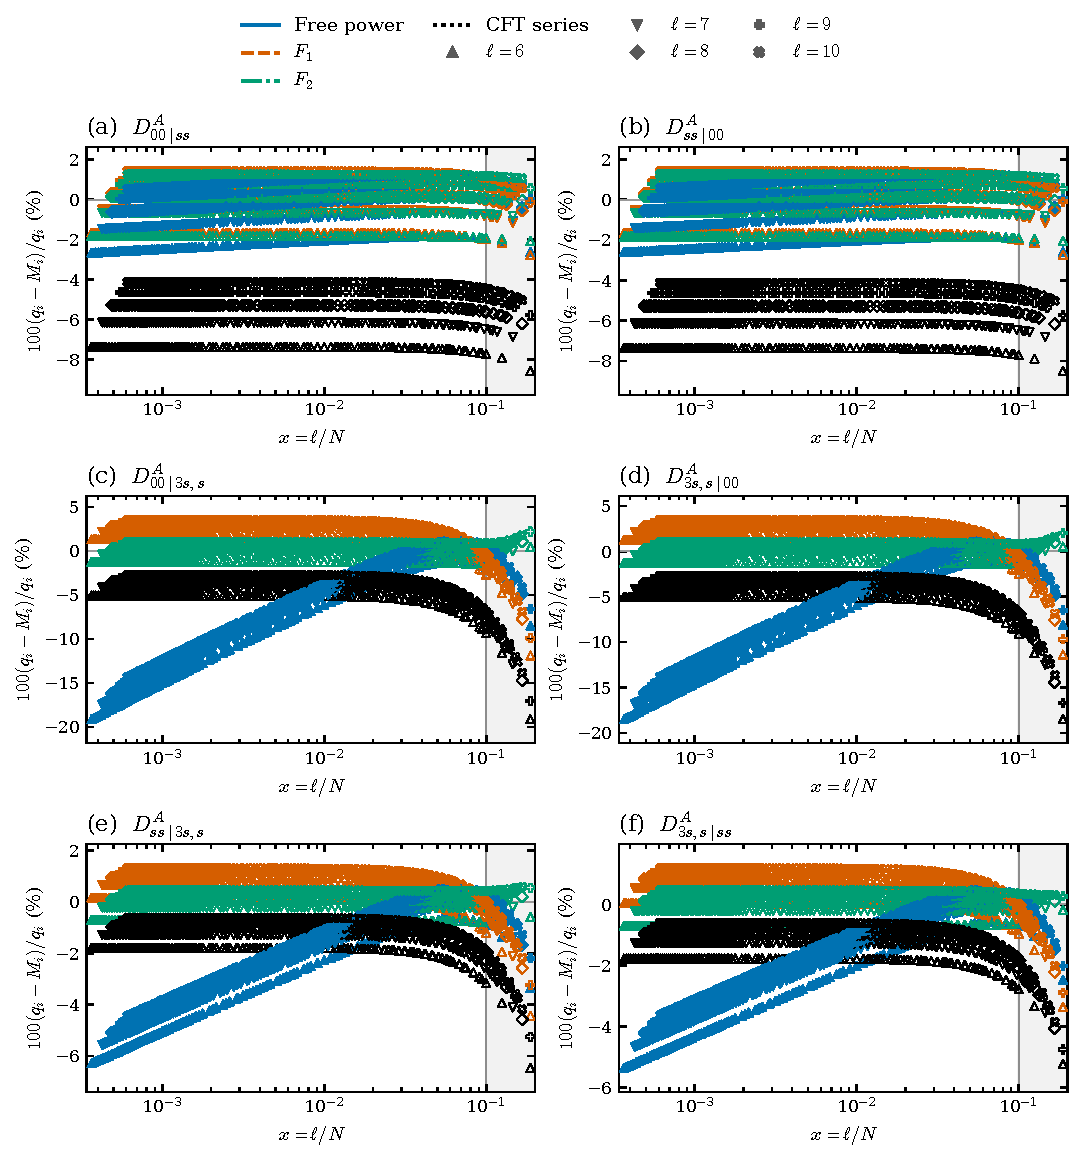
\includegraphics[width=.88\linewidth]{../figs/boson_small_residual.pdf}
\caption{The ordinate is $100(q_i-M_i)/q_i$ percent, with $q_i=D^A_i$ for a small interval and $q_i=\delta_i$ for a large interval; the horizontal zero line aids comparison. All four models have residual markers, colored as their curves. The residual ordinate is linear; the fraction axis is logarithmic. Compact-boson mixtures at $p=1/2$, $\ell=6,7,8,9,10$, and the chain-size set in Eq.~\eqref{eq:extended-grid}, with $32\leq N\leq16384$. There are 625 displayed geometries per direction at $x\leq0.2$, of which 598 satisfy $x\leq0.1$ and enter every fit. Marker shape identifies $\ell$; the vertical boundary and gray shading mark the fitting cutoff and excluded data. The boson uses $s=1/\sqrt2$, $q=2$, charge codes $(0,0),(1,1),(3,1)$, $z_j=e^{2\pi i j/N}$, $w_1=0$, and $W=10^8$; moment algebra uses 100 digits through $N=256$ and 120 digits at the added sizes. Natural logarithms apply. Added sizes use the direct entropy remainder in Sec.~\ref{sec:stable-entropy}, with support cutoff $10^{-15}$. Blue solid is the free-power fit (two fitted parameters), orange dashed is $F_1$ (one), green dash--dot is $F_2$ (two), and black dotted is the supplied CFT series (zero). Powers and amplitudes use Eqs.~\eqref{eq:fit} and \eqref{eq:hierarchy}; all coefficients include powers of $\pi$. Fits minimize unweighted squared residuals in $D^A$. These curves use \texttt{scaling\_fit\_summary.csv}. The identical fits in Tables~\ref{tab:boson-small-parameters} and \ref{tab:boson-small-metrics} also have per-pair full-range and fitting-window views in Sec.~\ref{sec:pair-small_boson}.}
\label{fig:bosonresid}
\end{figure}
